\section{Derefinement} \label{SEC_DEREFINEMENT}

Derefinement means the fusion of eight cells with the same level of
refinement $n$ and belonging to the same bunch back into a unique
cell of refinement level $n - 1$ (Figures
\ref{FIG_BEFORE_DEREFINEMENT} and \ref{FIG_AFTER_DEREFINEMENT}).

\begin{figure}[H]
    \centering
    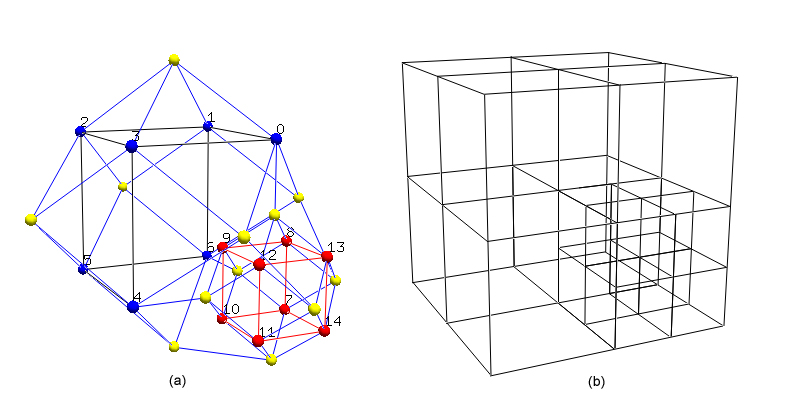
\includegraphics[scale=0.40]{../img/refinedGraphAndGrid.jpg}
    \caption{Graph and mesh before derefinement.}
    \label{FIG_BEFORE_DEREFINEMENT}
\end{figure}

\begin{figure}
    \centering
    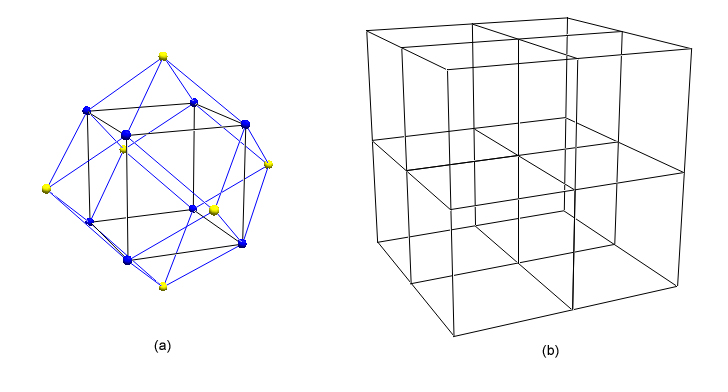
\includegraphics[scale=0.40]{../img/initialGraphAndGrid.jpg}
    \caption{Graph and mesh after derefinement.}
    \label{FIG_AFTER_DEREFINEMENT}
\end{figure}

The decision to derefine or not a bunch is taken according to
criteria established by the application. Generally, one derefines a
bunch when the variation in some physical variable within the cells
in a certain neighborhood is below some preset threshold. When this
happens, the number of cells in the region becomes greater than that
necessary in order to accomplish an accurate approximation of the
exact solution in that region, causing wastage of memory and
processing power.

\subsection{Mesh derefinement}
The derefinement of the mesh is done by the method
\textit{derefine()}. Whenever it is called upon, a research is done
on all cells of the mesh to determine which ones are qualified for
derefinement according to the criteria explained above.

Before a bunch is actually derefined, the cells initially qualified
for derefinement must pass some tests. First, all cells must belong
to the same bunch, otherwise it will not be allowed that the $8$
adjacent cells which define a cube in the mesh be derefined, even if
they satisfy the derefinement condition adopted by the application.
Second, all cells in the bunch must satisfy the derefinement
condition. Algorithm \ref{DEREFINEMENT_PROCEDURE} presented below
resumes what is done by method \textit{derefine()}. It receives as a
parameter the maximum variation accepted by one or more physical
variables upon which the derefinement is based.

\alglanguage{pseudocode}
\begin{algorithm}[!ht]
    \caption{Mesh derefinement}
    \small{
    \begin{algorithmic}[1]
    \Procedure{derefine}{maxPrecision}
        \State $CellNode \hspace{2mm} currentCell \gets firstCell$
        \State $CellNode \hspace{2mm} cellAfterBunch \gets currentCell$
        \While{$currentCell$ is not $null$}
            \If{$currentCell$ and its seven adjacent cells belong to the same bunch}
                \If{all cells of current bunch have the specified properties $>$ $maxPrecision$}
                    \State$cellAfterBunch \gets currentCell$
                    \For{i $\gets$ 0 \textbf{to} 8}
                         \State $cellAfterBunch \gets cellAfterBunch.next$
                     \EndFor
                    \State $derefineBunch(currentCell)$
                \EndIf
            \EndIf
            \State$currentCell \gets cellAfterBunch$
            \If{$cellAfterBunch$ is not $null$}
                \State$cellAfterBunch \gets cellAfterBunch.next$
            \EndIf
        \EndWhile
    \EndProcedure
    \end{algorithmic}
    }
    \label{DEREFINEMENT_PROCEDURE}
\end{algorithm}

Notice that in Line 5 the algorithm verifies if the current cell and
its seven adjacent cells belong to the same bunch. This happens when
they have the same refinement level and the division without
remainder of the attribute \textit{bunchNumber} of each cell wields
the same result.

Function \textit{derefineBunch()} called in Line 11 receives as a
parameter the first cell of the bunch to be refined. Its task is to
derefine the bunch, as will be discussed next.

\subsection{Bunch derefinement} \label{SUBSEC_PROCEDURE_DEREF}
The bunch derefinement procedure has as a parameter the first cell
of the bunch to be refined, as the mesh derefinement algorithm
encounters when it follows the ordering established by the Hilbert
curve. In order to obtain the remaining cells of the bunch, it just
follows the order given by the Hilbert curve until the seventh next
cell, because the Hilbert curve is built in such a way as to ensure
that all cells belonging to the same bunch follow in a sequence one
after the other in the chain list defined by the curve. Therefore,
is suffices to access the first cell of the list in order to obtain
access to the remaining cells of the bunch.

The entire process is divided below in six steps, each step
discussed in detail in the next paragraphs.

\begin{enumerate}
\item Creation of the cell node which will replace the bunch.
\item Creation of six transition nodes around the replacer cell node.
\item Linking between the cell and transition nodes just created.
\item Linking of the new transition nodes to the neighboring nodes of the bunch being derefined.
\item Elimination of all nodes of the bunch to be derefined.
\item Removal of unnecessary transition nodes in the neighborhood of the derefined bunch.
\end{enumerate}


\subsubsection*{Step 1. Creation of the cell node which replaces the bunch}
The derefinement procedure produces a cell with characteristics
which are similar to the cell which originated the bunch which is
being derefined. Its attributes are computed from the corresponding
attributes of the cells in the bunch. In the end, the group of eight
cells which form the bunch is replaced by the recently created cell.

In order to avoid the costs of memory allocation and management
associated with the creation of a new cell, one uses a preexistent
cell of the bunch to replace it. In this implementation, the front
northeast cell was chosen. Algorithm \ref{STEP_1_DEREFINEMENT}
(Lines 11 through 19) shows how this cell recovers some of the
geometric and topological attributes of the original cell that gave
origin to the bunch. Lines 12 through 14 reconfigure the geometric
coordinates. Line 15 computes the identifier of the replacer cell,
restoring it to the value of the cell which originated the bunch:
this identifier was built in such a way as to guarantee that all
cells belonging to the same bunch produce the same value when their
identifier is divided without remainder by 10 (see Step 2 in Section
\ref{SEC_REFINEMENT}). Line 16 computes the value of the basic form
of the Hilbert curve that will be attributed to the replacer cell;
this value is read by the refinement procedure, in case it is
decided in another iteration of the program that this cell must be
refined again, in order to tell how the cells of the resulting bunch
will be ordered by the Hilbert curve (see Section
\ref{SEC_HILBERT_CURVE}). This information is passed on by the cells
of the present bunch themselves, which give the replacer cell the
precise value so that in the future the cells of the newly refined
bunch should be ordered in the same way. This procedure is
fundamental for the correct functioning of the Hilbert curve. A call
to the function \textit{getFatherHilbertShape()} returns the number
of the Hilbert curve shape that was used in the refinement routine
for the ordering of the cells in the current bunch. Lines 17 and 18
update the refinement level and cell length, respectively. Other
variables which depend on the problem being considered should be
updated in this stage of the derefinement as well.

\alglanguage{pseudocode}
\begin{algorithm}[!ht]
    \caption{Step 1 of 6}
    \small{
    \begin{algorithmic}[1]
        \Procedure{derefineBunch}{firstBunchCell}
        \State $CellNode \hspace{2mm} frontNE \gets getFrontNortheastCell(firstBunchCell)$
        \State $CellNode \hspace{2mm} frontNW \gets frontNE.west$
        \State $CellNode \hspace{2mm} frontSE \gets frontNE.south$
        \State $CellNode \hspace{2mm} frontSW \gets frontNW.south$
        \State $CellNode \hspace{2mm} backNE \gets frontNE.back$
        \State $CellNode \hspace{2mm} backNW \gets backNE.west$
        \State $CellNode \hspace{2mm} backSE \gets backNE.south$
        \State $CellNode \hspace{2mm} backSW \gets backNW.south$
        \State
        \State $CellNode\hspace{2mm} replacerCell \gets frontNE$
        \State $replacerCell.x \gets (replacerCell.x + replacerCell.back.x) / 2$
        \State $replacerCell.y \gets (replacerCell.y + replacerCell.west.y) / 2$
        \State $replacerCell.z \gets (replacerCell.z + replacerCell.south.z) / 2$
        \State $replacerCell.bunchNumber \gets firstBunchCell.bunchNumber / 10$
        \State $replacerCell.HilbertShapeNumber \gets getFatherHilbertShape(firstBunchCell)$
        \State $replacerCell.level \gets firstBunchCell.level - 1$
        \State $replacerCell.side \gets cellNode.side * 2$
        \State updates other attributes.
        \State
        \State $CellNode\hspace{2mm} cellBeforeBunch \gets firstBunchCell.previous$
        \State $CellNode\hspace{2mm} cellAfterBunch \gets firstBunchCell$
        \For{i $\gets$ 0 \textbf{to} 8}
            \State $cellAfterBunch \gets cellAfterBunch.next$
        \EndFor
        \State $replacerCell.previous \gets cellBeforeBunch$
        \State $replacerCell.next \gets cellAfterBunch$
        \If{$replacerCell.previous$ is not null}
            \State $replacerCell.previous.next \gets replacerCell$
        \EndIf
        \If{$replacerCell.next$ is not null}
            \State $replacerCell.next.previous \gets replacerCell$
        \EndIf
        \algstore{derefinebunch}
    \end{algorithmic}
    }
    \label{STEP_1_DEREFINEMENT}
\end{algorithm}

It is necessary to store references for all cell nodes in the bunch.
This is done in Lines 2 through 9 in Algorithm
\ref{STEP_1_DEREFINEMENT}. In order to find out the front northeast
cell of the bunch, function \textit{getFrontNortheastCell()} is
called. Its determination is done analyzing the geometric
coordinates of all cells in the bunch.

The code from Lines 21 through 33 reconfigures the pointers
\textit{previous} and \textit{next} from the chain list defined by
the Hilbert curve. Since the cell nodes from the bunch will be
removed from the graph in the last stages of derefinement, it is
necessary that they be removed also from this chain list. The
removal action consists simply in substituting the replacer cell
node in place of the sublist of the bunch cells.

\subsubsection*{Step 2. Creation of the six transition nodes of the replacer cell node}
The replacer cell must have its directional pointers pointed to the
neighboring nodes of the bunch which is being derefined.  The
refinement level of these nodes may be different from the replacer
cell, making it necessary the existence of transition nodes for the
communication of nodes having different refinement levels. Therefore
a transition node is created for each direction. Notice that, if in
some direction the cells nodes have the same refinement level, no
transition node would be necessary in that direction. Nonetheless,
transition nodes are initially created in every direction; those
unneeded will be later removed in the simplification procedure (see
Step 6). Although in principle one could design the derefinement
procedure in such a way as not to create unnecessary transition
nodes from the start, this would unreasonably complicate matters,
making the algorithm difficult to understand and not gaining much in
terms of performance, since a simplifying procedure would be needed
anyway in order to get rid of unnecessary transition nodes present
in the neighborhood of the replaced bunch due to its neighboring
cells.

Figure \ref{FIG_DEREFINING} shows how the new transition nodes
(white circles) are related to the replacer cell and the replaced
bunch neighbors. The single connector of each node is pointed to the
replacer cell, while the quadruple connectors point to the
neighbors. Algorithm \ref{STEP_2_AND_3_DEREFINEMENT} shows how these
nodes are created. Note in Line 42 that the refinement level of each
transition node is configured to be one unit less than the
refinement level of the bunch, that is, to match the refinement
level of the replacer cell.


\begin{figure}[!hb]
    \centering
    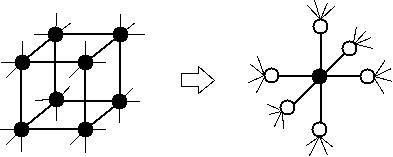
\includegraphics[scale=0.5]{../img/derefinement.jpg}
    \caption{Creation of transition nodes for the replacer cell.}
    \label{FIG_DEREFINING}
\end{figure}


\alglanguage{pseudocode}
\begin{algorithm}[!ht]
    \caption{Steps 2 and 3 of 6.}
    \small{
    \begin{algorithmic}[1]
        \algrestore{derefinebunch}
        \State $TransitionNode \hspace{2mm} northTN \gets \New \hspace{2mm} TransitionNode$
        \Comment{North node.}

        \State $TransitionNode \hspace{2mm} southTN \gets \New \hspace{2mm} TransitionNode$
        \Comment{South node.}

        \State $TransitionNode \hspace{2mm} eastTN \gets \New \hspace{2mm} TransitionNode$
        \Comment{ East node}.

        \State $TransitionNode \hspace{2mm} westTN \gets \New \hspace{2mm} TransitionNode$
        \Comment{ West node.}

        \State $TransitionNode \hspace{2mm} frontTN \gets \New \hspace{2mm} TransitionNode$
        \Comment{Front node.}

        \State $TransitionNode \hspace{2mm} backTN \gets \New \hspace{2mm} TransitionNode$
        \Comment{ Back node.}

        \State $ $
        \For{\textbf{each} new transition node}
            \State sets current node's refinement level to $firstBunchCell.level - 1$
            \State computes and sets current node's coordinates
            \State points current node's single connector to $replacerCell$
        \EndFor
        \State
        \State $replacerCell.north \gets northTN $
        \State $replacerCell.south \gets southTN $
        \State $replacerCell.east \gets eastTN $
        \State $replacerCell.west \gets westTN $
        \State $replacerCell.front \gets frontTN $
        \State $replacerCell.back \gets backTN $

        \algstore{derefinebunch}
    \end{algorithmic}
    }
    \label{STEP_2_AND_3_DEREFINEMENT}
\end{algorithm}


\subsubsection*{Step 3. Linking between the replacer cell node and its transition nodes}
After the creation of the transition nodes, it is necessary to link
them to the replacer cell. This consists simply in pointing the
single connector of each transition node to the replacer cell. Next,
each directional pointer of the replacer cell must be pointed to the
transition node located in the appropriate direction, i.e., north
pointer should be directed to the north transition node and so on.
In Algorithm \ref{STEP_2_AND_3_DEREFINEMENT}, the first operation is
executed in Line 44 while the second operation is executed in Lines
47 through 52.

\subsubsection*{Step 4. Linking between the replacer cell transition nodes and neighbor nodes of derefined bunch}
In this stage, the quadruple connectors of the transition nodes are
pointed to the neighboring nodes of the replaced bunch. The scheme
represented in Figure \ref{SCHEME_4CONNECTORS} is again used here to
ensure coherence. For instance, the quadruple connectors of the
north transition node must be pointed to the nodes pointed to by the
north directional pointers of each cell in the north face of the
bunch. According to the scheme of Figure \ref{SCHEME_4CONNECTORS},
the quadruple connectors 1, 2, 3 and 4 must be pointed to the north
neighbor node of the cells front northwest, front northeast, back
northeast and back northwest, respectively. These connections are
done by Algorithm \ref{STEP_4_DEREFINEMENT}.

\alglanguage{pseudocode}
\begin{algorithm}[!ht]
    \caption{Step 4 of 6}
    \small{
    \begin{algorithmic}[1]
        \algrestore{derefinebunch}
        \State $northTN.quadrupleConnector1 \gets frontNW.north $
        \State $northTN.quadrupleConnector2 \gets frontNE.north $
        \State $northTN.quadrupleConnector3 \gets backNE.north $
        \State $northTN.quadrupleConnector4 \gets backNW.north $
        \State
        \State $southTN.quadrupleConnector1 \gets frontSW.south $
        \State $southTN.quadrupleConnector2 \gets frontSE.south $
        \State $southTN.quadrupleConnector3 \gets backSE.south $
        \State $southTN.quadrupleConnector4 \gets backSW.south $
        \State
        \State $eastTN.quadrupleConnector1 \gets frontNE.east $
        \State $eastTN.quadrupleConnector2 \gets frontSE.east $
        \State $eastTN.quadrupleConnector3 \gets backSE.east $
        \State $eastTN.quadrupleConnector4 \gets backNE.east $
        \State
        \State $westTN.quadrupleConnector1 \gets frontNW.west $
        \State $westTN.quadrupleConnector2 \gets frontSW.west $
        \State $westTN.quadrupleConnector3 \gets backSW.west $
        \State $westTN.quadrupleConnector4 \gets backNW.west $
        \State
        \State $frontTN.quadrupleConnector1 \gets frontSW.front $
        \State $frontTN.quadrupleConnector2 \gets frontSE.front $
        \State $frontTN.quadrupleConnector3 \gets frontNE.front $
        \State $frontTN.quadrupleConnector4 \gets frontNW.front $
        \State
        \State $backTN.quadrupleConnector1 \gets backSW.back $
        \State $backTN.quadrupleConnector2 \gets backSE.back $
        \State $backTN.quadrupleConnector3 \gets backNE.back $
        \State $backTN.quadrupleConnector4 \gets backNW.back $
        \algstore{derefinebunch}
    \end{algorithmic}
    }
    \label{STEP_4_DEREFINEMENT}
\end{algorithm}

\subsubsection*{Step 5. Elimination of nodes of derefined bunch}
At this point, the replacer cell is completely built and properly
inserted in the graph. Therefore, the cells which made up the bunch
are no longer needed and must be removed from the graph. The removal
is straightforward and executed in the first lines of Algorithm
\ref{STEP_5_AND_6_DEREFINEMENT}. Notice that the front northeast
cell is not removed, since it was chosen in the beginning to become
the replacer cell.

\subsubsection*{Step 6. Removal of unnecessary transition nodes}
As in the refinement process, after the derefinement of a bunch
there may occur in the new graph transition nodes that connect cell
nodes with the same level of refinement. These cells serve no
purpose in the graph and must be eliminated. In order to do this,
each recently created transition node goes through a simplification
procedure, which identifies the unnecessary nodes and removes them.
Moreover, the simplification procedure makes the direct link between
cell nodes with the same refinement level and completes the
connection of the neighboring nodes of the replaced bunch to the
replacer cell (in Step 4, the quadruple connectors of each
transition node were pointed to the neighboring nodes but these
nodes did not point any of their directional nodes to the node which
pointed to them). Thus, beside eliminating needless transition
nodes, the simplification routine in the derefinement procedure also
completes the connection of the replacer cell to the graph. The
simplification routine for the derefinement procedure is explained
in detail in the next section.

\alglanguage{pseudocode}
\begin{algorithm}[ht]
    \caption{Step 5 of 6}
    \small{
    \begin{algorithmic}[1]
        \algrestore{derefinebunch}
        \State \textbf{delete} $\hspace{2mm} frontNW $
        \State \textbf{delete} $\hspace{2mm} frontSW $
        \State \textbf{delete} $\hspace{2mm} frontSE $
        \State \textbf{delete} $\hspace{2mm} backNE $
        \State \textbf{delete} $\hspace{2mm} backNW $
        \State \textbf{delete} $\hspace{2mm} backSE $
        \State \textbf{delete} $\hspace{2mm} backSW $
        \State
        \State $simplifyDeref(northTN)$
        \State $simplifyDeref(southTN) $
        \State $simplifyDeref(eastTN) $
        \State $simplifyDeref(westTN) $
        \State $simplifyDeref(frontTN) $
        \State $simplifyDeref(backTN) $
        \EndProcedure
    \end{algorithmic}
    }
    \label{STEP_5_AND_6_DEREFINEMENT}
\end{algorithm}

\subsection{Simplification routine} \label{SUBSEC_SIMPLIFICACAO_DESREF}
When a bunch is derefined, six transition nodes are created around
the replacer node. These nodes are connected to the replacer node
and the neighboring nodes of the replaced bunch. It may happen that
one of the neighboring cell nodes has the same refinement level as
the replacer cell. In this case, the two cell nodes must be directly
linked.

The connection between a replacer node and its neighbor can present
several different configurations, depending on the refinement levels
and types of its neighbors. Figure
\ref{FIG_SIMPLIFICATION_DEREFINEMENT} shows the three different
possible situations.

\vspace{1cm}
\begin{figure}[H]
    \centering
    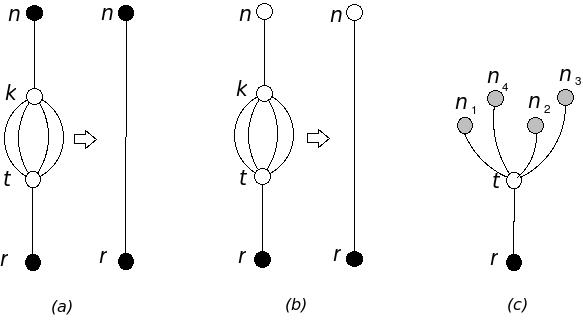
\includegraphics[scale=0.45]{../img/simplification_derefinement.jpg}
    \caption{Simplification through elimination of transition nodes.}
    \label{FIG_SIMPLIFICATION_DEREFINEMENT}
\end{figure}
\vspace{1cm}

In Figure \ref{FIG_SIMPLIFICATION_DEREFINEMENT}, the nodes denoted
by letters $r$, $t$ and $k$ are, respectively, the replacer cell
node, a transition node created during derefinement, and the
transition node which links to the neighbor node $n$ of the original
bunch.

The simplification procedure happens in the following manner:

\begin{enumerate}
 \item If node $r$ has the same refinement level as node $n$, as it
 happens in cases \textit{(a)} and \textit{(b)}, $r$ and $n$ are
 directly linked. Next, nodes $t$ and $k$ are removed from the graph. Notice that the difference between cases \textit{(a)}
 and \textit{(b)} is that in the first $r$ and $n$ have the same type, while in the latter $r$ is a cell node and
 $n$ is a transition node.

 \item If the quadruple connectors of $t$ point to different cells, then no simplification should be done,
 as in case \textit{(c)}, since this means that $n$ and the nodes $n_i$, $1 \leqslant i \leqslant 4$, have different refinement levels
 or are of different types.
\end{enumerate}

Algorithm \ref{SIMPLIFICATION_DEREFINEMENT} executes the simplifying
steps described above. In the third case, each node
$n_{i}$ must point to the transition node $t$. Notice that it is not
necessary to point $t$ to each node $n_{i}$, since this was already
done in Step 4.

The code from Line 13 through 15 does the simplification for case
\textit{(a)}. The pointer of $n$ (\textit{neighborCN}) which points
to $k$ (\textit{auxiliarTN}) must be modified to point to $r$
(\textit{replacerCell}). This pointer is that whose direction is
opposite to the direction of transition node $t$
(\textit{transitionNode}). The elimination of nodes $t$ and $k$
occurs in Lines 32 and 33, respectively.

The simplification of the second case is executed by the code in Lines
16 through 27. As in case \textit{(a)}, the pointer of $n$ (now
designated \textit{neighborTN}) that points to $k$ must be altered
to point to $r$. Since $n$ is a transition node and one cannot know
a priori which of its five pointers points to $k$, an inspection
must be obligatorily done on all pointers of $n$ to find out which
one points to $k$; once this is found, it is modified to point to
$r$. After the linking, nodes $t$ and $k$ are removed from the
graph.

In the third case, each node $n_i$ (designated by the vector
\textit{quadCon}) must point to the transition node $t$. These nodes
may be each either a cell node or a transition node. If it is a
transition node, its single connector is pointed to $t$; if it is a
cell node, the directional pointer whose direction is opposite to
the direction of $t$ is the one which is pointed to $t$. The
distinction between these two cases occurs in Lines 40 through 43.

\alglanguage{pseudocode}
\begin{algorithm}[!ht]
    \caption{Simplification - Derefinement}
    \small{
    \begin{algorithmic}[1]
    \Procedure{simplifyDeref}{transitionNode}
        \State $CellNode\hspace{2mm} replacerCell \gets transitionNode.singleConnector$
        \State $CellNode\hspace{2mm} neighborCN \gets null$
        \State $TransitionNode\hspace{2mm} neighborTN \gets null$
        \State $TransitionNode\hspace{2mm} auxiliarTN \gets null$
        \State $Cell\hspace{2mm} quadCon[4] \gets null$
        \State $char\hspace{2mm} direction \gets transitionNode.direction$

        \State
        \If{all transitionNode's quadruple connectors point to the same cell}
            \State $auxiliarTN \gets transitionNode.quadrupleConnector1$
            \State $replacerCell.getNeighborCell(direction) \gets auxiliarTN.singleConnector$
            \State $neighborType \gets auxiliarTN.singleConnector.type$
            \If{the neighbor cell is a cell node}
                \State $neighborCN \gets auxiliarTN.singleConnector$
                \State $neighborCN.oppositeDirection(direction) \gets replacerCell$
            \Else
                \State $neighborTN \gets auxiliarTN.singleConnector$
                \If{$neighborTN.singleConnector == auxiliarTN$}
                    \State $neighborTN.singleConnector \gets replacerCell$
                \ElsIf{$neighborTN.quadrupleConnector1 == auxiliarTN$}
                    \State $neighborTN.quadrupleConnector1 \gets replacerCell$
                \ElsIf{$neighborTN.quadrupleConnector2  == auxiliarTN$}
                    \State $neighborTN.quadrupleConnector2 \gets replacerCell$
                \ElsIf{$neighborTN.quadrupleConnector3 == auxiliarTN$}
                    \State $neighborTN.quadrupleConnector3 \gets replacerCell$
                \ElsIf{$neighborTN.quadrupleConnector4 == auxiliarTN$}
                    \State $neighborTN.quadrupleConnector4 \gets replacerCell$
                \Else
                    \State $print('Error')$
                \EndIf
            \EndIf
            \State \textbf{delete} $transitionNode$
            \State \textbf{delete} $auxiliarTN$
        \Else \Comment{In this case the neighbor cells are only linked, not simplified ($3^{\textrm rd}$ case)}
            \State $quadCon[0] \gets transitionNode.quadrupleConnector1$
            \State $quadCon[1] \gets transitionNode.quadrupleConnector2$
            \State $quadCon[2] \gets transitionNode.quadrupleConnector3$
            \State $quadCon[3] \gets transitionNode.quadrupleConnector4$
            \For{$i \gets 0$ \textbf{to} $3$}
                \If{$quadCon[i]$ is a transition node}
                    \State $neighborTN \gets quadCon[i]$
                    \State $neighborTN.singleConnector \gets transitionNode$
                \Else \Comment{the neighbor cell is a cell node}
                    \State $neighborCN \gets quadCon[i]$
                    \State $neighborCN.oppositeDirection(direction) \gets transitionNode$
                \EndIf
            \EndFor
        \EndIf
    \EndProcedure
    \end{algorithmic}
    }
    \label{SIMPLIFICATION_DEREFINEMENT}
\end{algorithm}
